\documentclass[a4paper]{report}

% \usepackage[utf8]{inputenc}
% \usepackage[T1]{fontenc}
% \usepackage{textcomp}
\usepackage[english]{babel}
\usepackage{amsmath, amssymb}
\usepackage[separate-uncertainty=true, multi-part-units=single]{siunitx}
\usepackage[]{subfig}
\usepackage[colorlinks=true, anchorcolor=blue, linkcolor=blue, citecolor=blue, bookmarks=false,hyperfootnotes=false]{hyperref}
\usepackage[margin=1in]{geometry}
\usepackage{color,soul}
\usepackage{tabularx}
% \usepackage[clean]{svg}


% figure support
\usepackage{import}
\usepackage{xifthen}
\pdfminorversion=7
\usepackage{pdfpages}
\usepackage{transparent}
\usepackage{physics}
\graphicspath{ {./figures/} }
% \setlength{\parindent}{0pt}
\usepackage{chngcntr}
\usepackage{verbatim}
\usepackage{indentfirst}
\numberwithin{equation}{section}
\counterwithin{figure}{section}
\newcommand{\incfig}[1]{%
		\def\svgwidth{\columnwidth}
		\import{./figures/}{#1.pdf_tex}

}

\pdfsuppresswarningpagegroup=1

% for citations / references
\usepackage[style=ieee]{biblatex}
\addbibresource{lasers_report.bib}

\begin{document}

%----------------------------------------------------------------------------------------
%	TITLE PAGE
%----------------------------------------------------------------------------------------
\begin{titlepage} % Suppresses displaying the page number on the title page and the subsequent page counts as page 1
	\newcommand{\HRule}{\rule{\linewidth}{0.5mm}} % Defines a new command for horizontal lines, change thickness here
	
	\center % Centre everything on the page
	%------------------------------------------------
	%	Headings
	%------------------------------------------------
	
	\textsc{\LARGE Rheinische Friedrich-Wilhelms-Universit\"at Bonn }\\[4cm] % Main heading such as the name of your university/college
	
	\textsc{\Large Advanced Laboratory Course}\\[0.5cm] % Major heading such as course name
	
	\textsc{\large Performed on: April 4th - 5th, 2022}\\[0.5cm] % Minor heading such as course title

	\textsc{\large Submitted on: May 3, 2022}\\[0.5cm] % Minor heading such as course title
	
	%------------------------------------------------
	%	Title
	%------------------------------------------------
	
	\HRule\\[0.4cm]
	
	{\huge\bfseries A249: Laser Gyroscope}\\[0.4cm] % Title of your document
	
	\HRule\\[1.5cm]
	
	%------------------------------------------------
	%	Author(s)
	%------------------------------------------------
	
	\begin{minipage}{0.4\textwidth}
		\begin{flushleft}
			\large
			\textit{Authors}\\
			Paarth Thakkar \\
			Keito Watanabe
		\end{flushleft}
	\end{minipage}
	~
	\begin{minipage}{0.4\textwidth}
		\begin{flushright}
			\large
			\textit{Tutor(s)}\\
			Thorsten Groh \\
			Marc Vöhringer
		\end{flushright}
	\end{minipage}

	\vspace*{5em}

	\begin{minipage}{0.8\textwidth}
		\begin{centering}
			% \large
			\textbf{Abstract}\\[0.2cm]
			 
		\end{centering}
	\end{minipage}
	
	% If you don't want a supervisor, uncomment the two lines below and comment the code above
	%{\large\textit{Author}}\\
	%John \textsc{Smith} % Your name
	
	%------------------------------------------------
	%	Date
	%------------------------------------------------
	
	%\vfill\vfill\vfill % Position the date 3/4 down the remaining page
	% \vfill\vfill
	
	% {\large\today} % Date, change the \today to a set date if you want to be precise
	
	%------------------------------------------------
	%	Logo
	%------------------------------------------------
	
	%\vfill\vfill
	%\includegraphics[width=0.2\textwidth]{placeholder.jpg}\\[1cm] % Include a department/university logo - this will require the graphicx package
	 
	%----------------------------------------------------------------------------------------
	
	% \vfill % Push the date up 1/4 of the remaining page
	
\end{titlepage}



\tableofcontents

\chapter{Introduction}

\chapter{Theory}

\section{Gyroscopes}

\subsection{The Sagnac Effect}

The Sagnac effect tells us that whilst the motion between two inertial frames cannot be distinguished, two rotating frames can be 
distinguished, allowing one to directly measure the rotation rate of an inertial system \cite{Groh2021}. This effect was first observed by 
George Sagnac in 1913, whom believed that this experiment was a proof that aether exists in an inertial frame  \cite{Darrigol2014}. This, however, was 
disproven by Max von Laue in 1911 where he showed that the Sagnac effect was compatible with special relativity \cite{Laue1911}. 
However, the interpretation of the Sagnac effect due to the general theory of relativity is still investigated today, 
even though it is already well-known in literature \cite{Benedetto2019}. In our analysis, we utilize the Sagnac effect on a gyroscope to 
measure the rotation rate of the Earth.\par

To observe the Sagnac effect, we consider an interferometer setup with light propagating with wavelength $\lambda$ enclosing an area $\vec{A}$
 with perimeter $P$. Placing such a setup onto a rotating platform with frequency $\vec{\Omega}$, we observe that the optical path that
 each light travels changes. For example, if the table rotates counter-clockwise, then the path of the co-rotating light increases, while that of the other light
decreases (see Fig. \ref{fig:sagnac_effect}). The Sagnac effect then tells us the resulting phase shift between the two lights:
\begin{equation}
	\delta \phi = \frac{8\pi \vec{A} \cdot \vec{\Omega}}{c \lambda} \propto \vec{A} \cdot \vec{\Omega}
\end{equation} 

\begin{figure*}[h!]
	\centering
	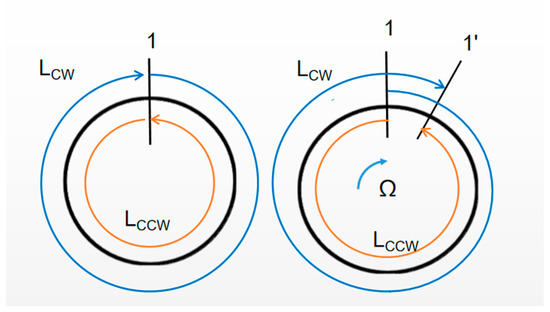
\includegraphics[width=0.6\columnwidth]{sagnac_effect.jpg}
	\caption{The Sagnac effect. \textit{Left}: Setup without rotation. The beam moving clockwise (blue) and counter-clockwise (orange)
	have the same optical path length. \textit{Right}: Setup with a clockwise rotation $\Omega$. The path length of the 
	clockwise beam is larger than that of the counter-clockwise beam \cite{Feng2020}.}
	\label{fig:sagnac_effect}
\end{figure*}

A more detailed derivation using the relativistic law of velocity addition can be found in Ref. \cite{Benedetto2019}. 

\subsection{Ring Laser Gyroscopes}

\subsubsection{Active Ring Laser Gyroscopes}

In order to incorporate the Sagnac effect within our experiment, we utilize ring laser gyroscopes. A laser is placed within an 
enclosed cavity, and emits two counter-propagating beams. Such beams reflect off mirrors and interfere at the end of their 
propagation. When rotating the platform in which such setup is placed, different interference patterns can be observed, and 
transforms the ring cavity system into a cavity resonator. The corresponding beat frequency $\delta \nu$ observed is then the 
Sagnac frequency, which is given as such:

\begin{equation}
	\delta \nu = \frac{4 \vec{A} \cdot \vec{\Omega}}{P \lambda}
	\label{eq:sagnac_freq}
\end{equation}

In our experiment, we only consider square ring cavities so that $A = L^2$ and $P = 4L$, where $L$ is the path length of each arm. 
As such, we can simplify Eq. \ref{eq:sagnac_freq} as such: 
\begin{equation}
	\delta \nu  = \frac{L \Omega}{\lambda} = n \Omega
\end{equation}
where $n = L / \lambda$ is the number of nodes of the light field in each arm. Thus the Sagnac frequency is proportional to the rotation rate
of the inertial system \cite{Groh2021}.\par 

\subsubsection{Passive Ring Laser Gyroscopes}

In contrast to the active ring laser gyroscope, in which the laser is contained within the ring cavity, the passive ring laser
gyroscope places the laser source outside of the cavity system. In this system, the external laser is locked to the counter-propagating
modes of the resonator. By placing the laser outside of the resonator, we can reduce the systematic effects due to the lasing medium and 
the lock-in effect (see Sec. \ref{sec:lockin_effect}), and also increase the available light power for the beam. 
This method, however, also introduces an added complexity of laser locking \cite{Groh2021}. See Fig. \ref{fig:passive_active} for a comparison between the two
systems. In our experiment, we use the passive ring laser gyroscope and thus laser locking becomes an importance in our measurements.

\begin{figure*}[h!]
	\centering
	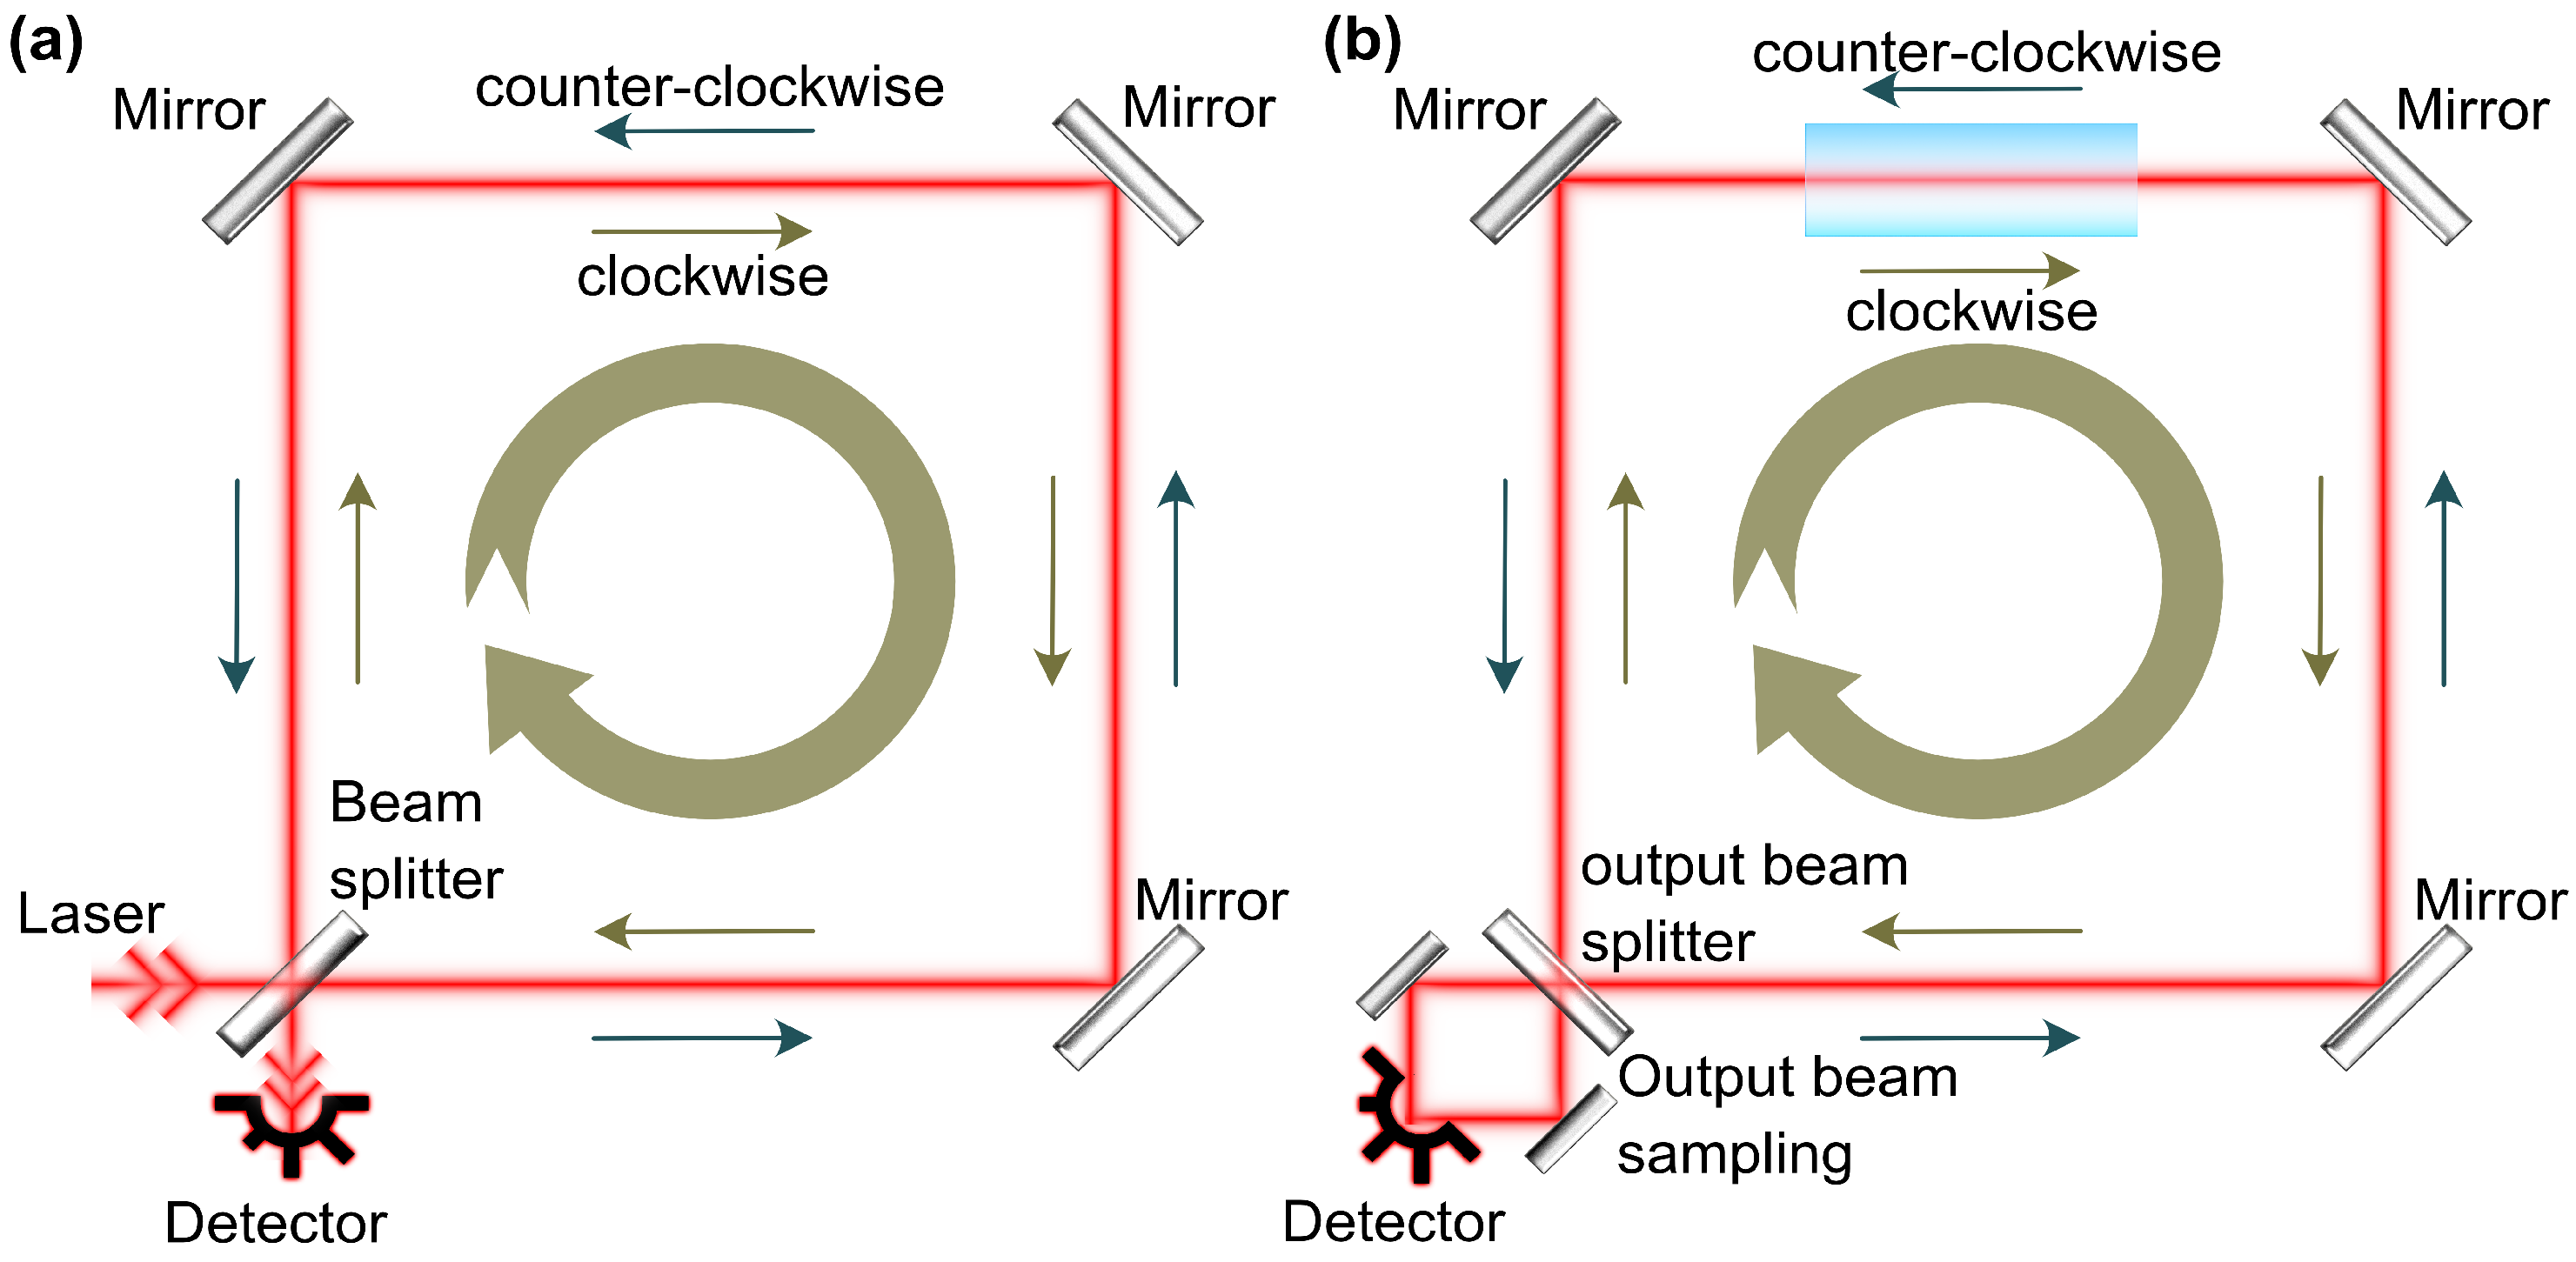
\includegraphics[width=0.6\columnwidth]{passive_active_gyroscope.png}
	\caption{A \textit{Left}: passive and \textit{Right}: active ring laser gyroscope system \cite{Kudelin2021}.}
	\label{fig:passive_active}
\end{figure*}

\subsubsection{Gyroscope Sensitivity}

The sensitivity of the ring laser gyroscope depends on a variety of factors, namely the wavelength $\lambda$, arm length $L$, finesse $F$
of the resonator (see Sec. \ref{sec:finesse}), and the shot-noise limited detection given by the number of photons $N = P_{\text{opt}} / h \nu = P_{\text{opt}} \lambda / hc$ detected per unit time. 
$P_{\text{opt}}$ represents the optical power given to the laser. Combining all such factors, we obtain the sensitivity of the ring laser gyroscope for an integration time $\tau$ as such: 
\begin{equation}
	\delta \Omega = \frac{1}{4} \frac{c}{L^2F}\sqrt{\frac{ch\lambda}{P_{\text{opt}}}} \frac{1}{\tau}
	\label{eq:gyroscope_sensitivity}
\end{equation}

This gyroscope sensitivity can be directly compared with the Allan deviation $\sigma_{\text{ad}}$ that determines the instability of 
a measurement for some averaged integration time $\tau$ (see Sec. \ref{sec:allan_dev}). The best gyroscope sensitivity observed was from the G-ring at the German
Fundamentalstation Wettzell with a sensitivity of around 12 prad / s / $\sqrt{\text{Hz}}$ \cite{Groh2021}. 

\section{Optical Cavities}

\subsection{Finesse} \label{sec:finesse}

\subsection{Lock-In Effect} \label{sec:lockin_effect}


\section{Allan Deviation} \label{sec:allan_dev}



\chapter{Pre-Lab Exercises}

Before conducting the experiment, we were required to determine the rotation rate of the Earth using our phone. Our phones
contain a microelectromechanical system (MEMS), which is a portable and inexpensive inertial sensor that track the motion of
the phone. Using the application \texttt{phyphox} constructed by RWTH Aachen University, we evaluated the capabilities
of the MEMS gyroscope within the iPhone 13. 

\chapter{Set-up and Procedure}

\chapter{Results and Discussion}

\chapter{Conclusion and Outlook}

\chapter{Acknowledgements}

\chapter{Appendix}

\end{document}